\chapter[Referencial Tecnológico]{Referencial Tecnológico}

Este capítulo apresenta as principais ferramentas e tecnologias utilizadas na realização deste trabalho. Para melhor organização, elas foram agrupadas de acordo com sua finalidade no projeto, contemplando recursos de apoio à produção acadêmica e à pesquisa, prototipação, desenvolvimento da aplicação, armazenamento de dados e ferramentas auxiliares.

A Figura \ref{fig:nuvem-tecnologias} apresenta uma nuvem de palavras com as principais tecnologias e ferramentas previstas para este trabalho. O tamanho de cada termo representa o grau de responsabilidade esperado da tecnologia no desenvolvimento do projeto, enquanto as cores indicam sua finalidade: azul para tecnologias centrais, verde para tecnologias complementares, roxo para infraestrutura e cinza para ferramentas auxiliares. Essa classificação foi definida pelos autores com base na participação prevista de cada tecnologia na solução proposta.

\begin{figure}[htbp]
    \centering
    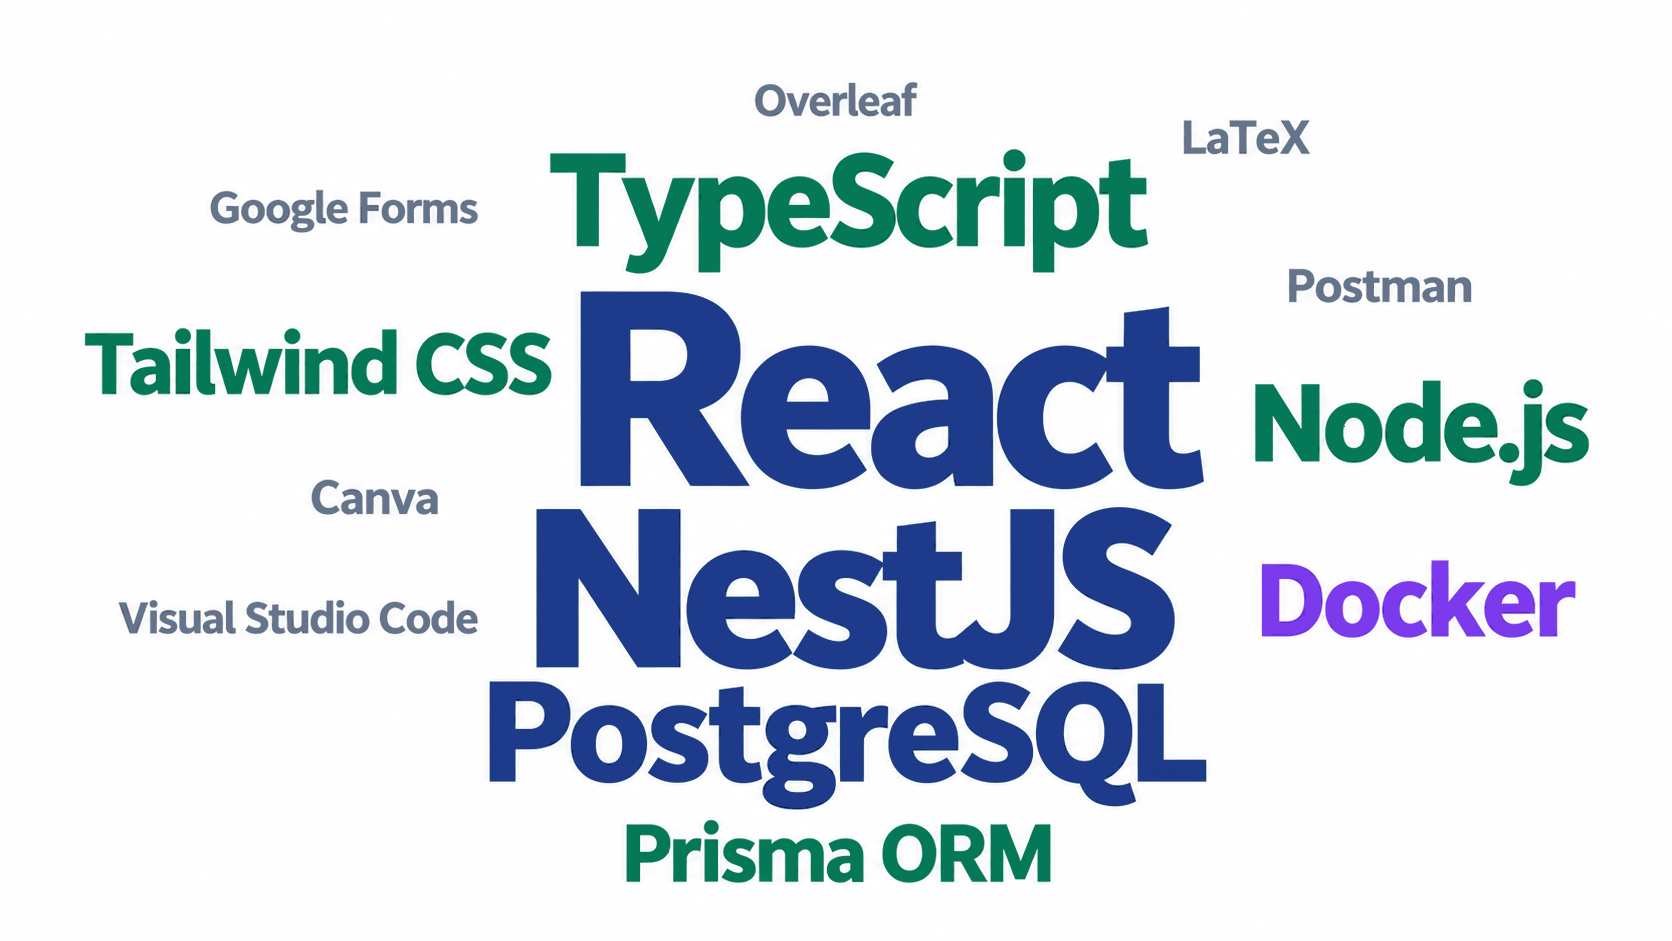
\includegraphics[width=0.85\textwidth]{figuras/nuvem-tecnologica.png}
    \caption{Nuvem de palavras das tecnologias previstas para o projeto}
    \label{fig:nuvem-tecnologias}
    \fonte{Elaboração própria (2026).}
\end{figure}


\section{Ferramentas de Apoio à Produção Acadêmica e à Pesquisa}

A elaboração deste documento foi realizada em \textbf{LaTeX}, um sistema de preparação de documentos utilizado na produção de textos técnicos e científicos, que permite estruturar elementos como capítulos, figuras, tabelas e referências bibliográficas de maneira padronizada. A edição foi feita por meio do \textbf{Overleaf}, uma plataforma online para criação e compilação de documentos LaTeX no navegador, dispensando a configuração de um ambiente local.

Para o levantamento de requisitos, será utilizado o \textbf{Google Forms}, ferramenta online para criação e aplicação de formulários e questionários. Por intermédio dela serão coletadas informações sobre as necessidades e dificuldades de estudantes, orientadores e coordenação no processo de TCC, cujos resultados auxiliarão na definição dos requisitos do sistema.

O \textbf{Canva} e o \textbf{GIMP} são ferramentas utilizadas para criação e edição de elementos visuais. O Canva é uma plataforma online de design gráfico, enquanto o GIMP é um software livre de edição e manipulação de imagens. Neste trabalho, ambas as ferramentas serão utilizadas na elaboração e edição de diagramas, figuras e outros elementos visuais que compõem o documento acadêmico.

\section{Prototipação e Desenvolvimento da Aplicação}

Antes da implementação definitiva, será desenvolvido um protótipo de alta fidelidade das telas e dos fluxos de interação do sistema, utilizando as mesmas tecnologias previstas para a aplicação final. Essa abordagem permite obter uma representação navegável e próxima do produto real, possibilitando a validação das interfaces junto aos usuários antes da implementação completa das funcionalidades, além de permitir o reaproveitamento de parte do código gerado durante a prototipação. 

A aplicação será desenvolvida em \textbf{TypeScript}, linguagem baseada em JavaScript que acrescenta recursos de tipagem estática. A utilização será utilizado tanto no frontend quanto no backend, contribuindo para a padronização do desenvolvimento e para a definição das estruturas de dados utilizadas pela aplicação. 

No frontend, será utilizado o \textbf{React}, biblioteca JavaScript que permite construir interfaces por meio de componentes reutilizáveis. A biblioteca utiliza JSX, uma extensão de sintaxe que possibilita escrever estruturas semelhantes ao HTML junto à lógica dos componentes. A estilização será realizada com o \textbf{Tailwind CSS}, framework baseado em classes utilitárias que facilita a implementação de interfaces responsivas.

No backend, será utilizado o \textbf{Node.js}, ambiente de execução JavaScript utilizado, entre outras finalidades, no desenvolvimento de aplicações no lado do servidor, em conjunto com o \textbf{NestJS}, framework que oferece suporte nativo ao TypeScript e uma estrutura modular para a organização do código. A partir dessas tecnologias serão implementadas a API REST e as regras de negócio do sistema.

\section{Armazenamento de Dados e Apoio ao Desenvolvimento}

Os dados da aplicação serão armazenados no \textbf{PostgreSQL}, sistema gerenciador de banco de dados relacional. O \textbf{Prisma ORM} será responsável pela comunicação entre o backend e o banco de dados, permitindo realizar operações de consulta e manipulação das informações armazenadas.

O editor de código-fonte \textbf{Visual Studio Code} será utilizado como ambiente principal para o desenvolvimento do frontend e do backend da aplicação. Os endpoints disponibilizados pela API serão testados com o 
\textbf{Postman}, ferramenta utilizada para desenvolvimento e teste de APIs. Por fim, o \textbf{Docker} será usado para executar a aplicação e seus serviços em contêineres, padronizando o ambiente de execução dos componentes do sistema e facilitando sua configuração durante o desenvolvimento.